\bundlefile{lecturesight-framesource-impl.jar}

The FrameSource bundle provides the infrastructure responsible for managing FrameSource implementations. It discovers video input plugins and is responsible for setting up \textit{FrameSources} with the propper input plugin. It also registers the \textit{FrameSourceProvider} service on startup, which is the point in the system where other services get the (masked) input image from the overview camera.

\configproperties

\property{cv.lecturesight.framesource.input.mrl}{v4l:///dev/video0[width=320;height=240]}{
MRL of the video input from the overview camera that is served by the FrameSourceProvider. The MRL must have the following form:

\begin{center}
{\tt type :// path [options] }
\end{center}

\noindent With

\begin{tabularx}{\textwidth}{rl}
{\tt type} & the type of the input, determines which input plugin is used\\
{\tt path} & path to the input, usually a linux device or file\\
{\tt options} & additional arguments for the input plugin
\end{tabularx}\\~\\
\noindent For example, the default value for this property tells the system to use the Video4Linux device \texttt{/dev/video0} as the overview source with QVGA resolution.
}

\property{cv.lecturesight.framesource.input.mask}{none}{
The path to the input mask image file for masking the input provided by the \textit{FrameSourceProvider}. The masking is deactivated if value is \texttt{none}. Otherwise the provided mask image is laoded when the framesource is activated and the mask is applied to each input frame before it is made availabel to consuming services: Each pixel in the input frame is set to black if the first component of the color value of the corresponding pixel in the mask image equals 0.\\

\image{img-framesource-mask}{A mask image}{
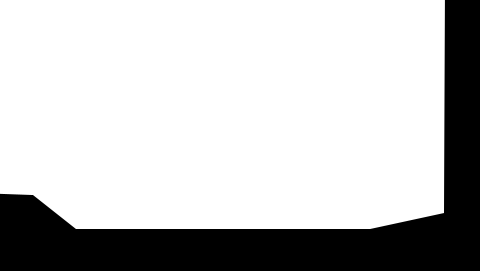
\includegraphics[width=0.5\textwidth]{../modules/lecturesight-framesource-impl/manual/mask.png}
}

\image{img-framesource-output}{A masked input frame}{
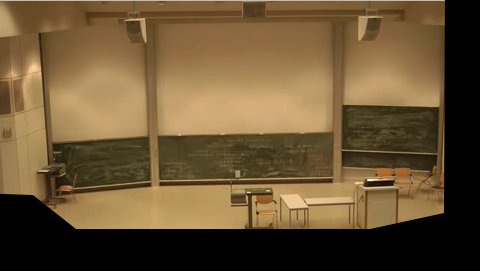
\includegraphics[width=0.5\textwidth]{../modules/lecturesight-framesource-impl/manual/output.png}
}

\noindent The following constraints apply to mask image files:

\begin{itemize}
 \item the file format must be either PNG or JPEG
 \item the dimensions of the mask image must be at leat those of the video input
 \item for a masking pixel the first component of the color value must equal 0
\end{itemize}
}
